\section{Технологическая часть}

Данный раздел содержит обоснование выбора средств программной реализации разработанного метода и описание программной реализации разрабатываемого метода. Приводится схема взаимодействия модулей разрабатываемого программного обеспечения. Описываются входные и выходные данные. Приводится методика тестирования модулей системы.



\subsection{Выбор средств программной реализации}

Для программной реализации поставленной необходимо прежде всего выбрать языки программирования как узлов, так и смарт-контрактов сети блокчейн. Также следует выбрать среду разработки проекта и библиотеку для написания узлов сети.


\subsubsection{Выбор языка программирования}

В качестве языка программирования узлов сети был выбран язык Rust по следующим причинам:
\begin{itemize}[leftmargin=1.6\parindent]
	\item[---] в Rust отсутствует <<сборщик мусора>>, что означает невозможность не детерминистических инцидентов (вызванных непосредственно языком) в ходе исполнения программы \cite{rust};
	\item[---] данный язык программирования содержит большое количество библиотек, упрощающих разработку узлов сети блокчейн;
	\item[---] имеется достаточный опыт программирования на этом языке, что сократит время написания программы.
\end{itemize}

В качестве языка программирования смарт-контрактов был выбран язык Solidity, поскольку:
\begin{itemize}[leftmargin=1.6\parindent]
	\item[---] он был спроектирован и создан как язык для написания смарт"=контрактов;
	\item[---] данный язык исполняется на специализированной виртуальной машине EVM \cite{evm}, абстрагируясь от реализации узлов сети \cite{solidity}.
\end{itemize}



\subsubsection{Выбор среды разработки}

В качестве среды разработки была выбрана редактор кода <<VS Code>> \cite{vscode}. Этот выбор обусловлен следующими причинами:
\begin{itemize}[leftmargin=1.6\parindent]
	\item[---] данный редактор кода свободно распространяется;
	\item[---] он содержит множество доступных плагинов платформы, которые существенно облегчают и ускоряют процесс написание кода.
\end{itemize}


\subsubsection{Выбор библиотеки для написания узлов сети}

Для создания узлов блокчейн-сети был выбран фреймворк Substrate, поскольку он написан на языке Rust и позволяет создавать гибкие и настраиваемые блокчейны \cite{substrate}. К тому же, данный фреймворк поддерживается активным сообществом разработчиков, что упрощает процесс разработки и изучения его документации.





\subsection{Структура разработанного ПО}

Блокчейн представляет из себя одноранговую сеть, то есть в ней отсутствуют <<центральные>> узлы. На рисунке \ref{fig:a8} приведена схема полносвязной одноранговой сети, состоящей из 5 участников.

\begin{figure}[hbtp]
	\centering
	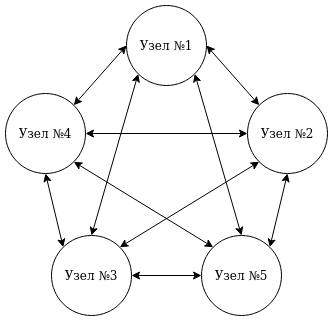
\includegraphics{img/p2p.png}
	\caption{Одноранговая сеть}
	\label{fig:a8}
\end{figure}

Чтобы выполнить поставленную задачу, необходимо реализовать узел сети блокчейн. Также следует написать смарт-контракт создания невзаимозаменяемых токенов в сети, который загружается в сеть. Для взаимодействия с сетью, требуется приложение-клиент.

%\subsubsection{Модули системы}

Разработанная система состоит из следующих модулей:
\begin{itemize}[leftmargin=1.6\parindent]
	\item[---] узел сети;
	\item[---] смарт-контракты;
	\item[---] браузерное клиентское приложение.
\end{itemize}

На каждом узле сети установлена специализированная виртуальная машина (в частности, EVM), которая обрабатывает транзакции пользователей: создание сертификата в сети и т.п. Помимо виртуальной машины узел также хранит актуальное состояние сети. Для взаимодействия с сетью необходимо, чтобы узел имел открытый порт для внешнего подключения; стандартным протоколом <<общения>>  является JSON-RPC \cite{rpc}. На рисунке \ref{fig:a9} приведена схема описанного взаимодействия.


\begin{figure}[hbtp]
	\centering
	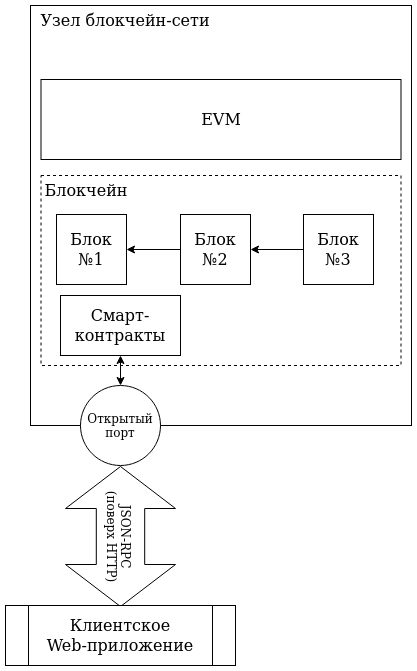
\includegraphics{img/node.png}
	\caption{Схема взаимодействия узла сети и клиентского приложения}
	\label{fig:a9}
\end{figure}



\subsubsection{Узел сети}

Как было упомянуто выше, для реализации узла сети был использован фреймворк Substrate. Для имплементации протокола консенсуса и EVM, необходимо настроить т.н. <<среду исполнения>> Substrate-узла: требуется сконфигурировать <<FRAME-паллеты>> Substrate, в частности, pallet\_aura и pallet\_grandpa для имплементации протокола консенсуса, а также pallet\_evm и pallet\_ethereum для поддержки EVM и смарт-контрактов в сети. В приложении A на листинге \ref{list1} приведен код настройки узла сети.


\subsubsection{Смарт-контракты}

Каждое учебное заведение владеет собственной копией смарт-контракта, который производит невзаимозаменяемые токены. Чтобы не плодить бесконтрольно копии смарт-контрактов, был реализован контракт-фабрика, который производит однотипные копии контрактов. Контракт-фабрика хранит адрес шаблонного контракта, который имплементируется для каждого учебного заведения. В приложении А на листинге \ref{list2} представлен код контракта-фабрики.

Смарт-контракт учебного заведения отвечает за создание и чтение сертификатов, созданных заведением, которое им владеет. Данный смарт-контракт имеет следующие поля, указанные в таблице 4.

\begin{table}[h!]
	\captionsetup{justification=raggedleft,singlelinecheck=off}
	\caption{Поля смарт-контракта учебного заведения}
	\resizebox{\columnwidth}{!}{\begin{tabular}{| p{6cm} | p{9cm}  |}
			\hline
			Название и тип поля & Описание поля \\
			\hline
			Название учебного заведения: string storage & Удобное для восприятия пользователя название учебного заведения (не более 255 символов) \\
			\hline
			Идентификатор токенов: Counter & Счетчик-идентификатор созданных токенов (начиная с 1) \\
			\hline
			URI токенов: отображение uint256 на string & Отображение идентификатор токенов на ссылки подтверждаемых документов \\
			\hline
	\end{tabular}}
\end{table}

Каждый созданный невзаимозаменяемый токен содержит в своих метаданных адрес владельца (выпускника), название учебной организации, которая выдала этот сертификат, а также ссылку на подтверждаемый документ. Хранение ссылки на документ вместо самого файла обусловлена дороговизной хранения данных в блокчейне: новым участникам сети придется скачивать больше данных, чтобы иметь актуальную версию блокчейна -- повышается нагрузка на сеть и требуется больше свободного места на машине \cite{ru-bchain4}.

Поскольку выпуск сертификатов должен быть доступен только владельцу контракта (учебному заведению), необходимо сконфигурировать доступ к методам контракта, путем расширения стандартных контрактов OpenZeppelin, таких как Ownable и AccessControl \cite{openzeppelin}.

В приложении А на листинге \ref{list3} приведен код смарт-контракта учебного заведения.




\subsubsection{Клиентское приложение}

С помощью библиотеки ethers.js было написано клиентское Web"=приложение \cite{ethersjs}. На каждой HTML-странице приложения содержится JS-скрипт, который при необходимости подключается к блокчейн"=сети под адресом пользователя. Имея ABI смарт"=контрактов и их адреса в сети, можно вызывать методы контрактов по протоколу JSON-RPC, которые доступны данному пользователю.

В приложении А на листинге \ref{list4} представлен код создания и чтения сертификата.






\subsection{Методика тестирования разработанных модулей}

Существуют три основных уровня тестирования разработанного
программного обеспечения:
\begin{itemize}[leftmargin=1.6\parindent]
	\item[---] Модульное тестирование — тестируется минимально возможный для тестирования компонент, например, отдельный класс или функция. Часто модульное тестирование осуществляется разработчиками программного обеспечения.
	\item[---] Интеграционное тестирование — тестируются интерфейсы между компонентами, подсистемами или системами. При наличии резерва времени на данной стадии тестирование ведётся итерационно, с постепенным подключением последующих подсистем.
	\item[---] Системное тестирование — тестируется интегрированная система на её соответствие требованиям.
\end{itemize}


Для тестирования разработанного ПО были написаны модульные тесты -- с помощью среды Hardhat \cite{hardhat} были протестированы методы смарт-контрактов, в частности, инициирования смарт-контракта учебного заведения, а также создания и чтения невзаимозаменяемого токена. Также в рамках системного тестирования была протестирована блокчейн-сеть на предмет достижения консенсуса и финализации цепочек блоков.




\subsection{Форматы входных и выходных данных}

Чтобы создать смарт-контракт организации в сети, необходимо ввести названии заведения. В ответ будет получен 42-символьный шестнадцатеричный адрес созданного смарт-контракта.

Входными данными для создания невзаимозаменяемого токена являются ссылка на документ об образовании, адрес смарт-контракта учебной организации, и адрес выпускника. Выходными данными будут являться ID созданного сертификата.
Для проверки сертификата необходимы ID токена и адрес смарт-контракта организации, которая выдала его. Вывод будет содержать метаданные сертификата, в случае если он существует, иначе сообщение об ошибке.


Входные данные:
\begin{itemize}[leftmargin=1.6\parindent]
	\item[---] название учебного заведения;
	\item[---] метаданные сертификата (ссылка на документ, адрес выпускника);
	\item[---] адрес смарт-контракта учебной организации;
	\item[---] ID сертификата.
\end{itemize}

Выходные данные:
\begin{itemize}[leftmargin=1.6\parindent]
	\item[---] адрес созданного смарт-контракта учебного заведения;
	\item[---] ID выпущенного сертификата;
	\item[---] метаданные проверяемого сертификата.
\end{itemize}




\subsection{Информация, необходимая для сборки и запуска}

Минимальные технические требования для машины подобраны с учётом, минимальных системных требований к Substrate-проектам \cite{substrate}:
\begin{itemize}[leftmargin=1.6\parindent]
	\item[---] четырехъядерный центральный процессор;
	\item[---] 8 гигабайт оперативной памяти;
	\item[---] 50 гигабайт свобдного места на HDD/SSD машины.
\end{itemize}




\subsection*{Выводы}
\addcontentsline{toc}{subsection}{Выводы}

В данном раздела было дано обоснование выбора средств реализации разрабатываемого метода. Была описана структура и схема взаимодействия модулей разрабатываемого программного обеспечения. Было дано описание входных и выходных данных для различных сценариев использования ПО; методика тестирования узлов и смарт"=контрактов сети. Также были представлены минимальные технические требования для запуска ПО.

\pagebreak